% Save this file as assignment2.tex
% Create plot1.eps, plot2.eps, plot3.eps in R, using function calls like
%    dev.copy2eps(file="plot1.eps")
% latex assignment2
% latex assignment2  (do twice for figure references and contents)
% dvips -o assignment2.ps -Ppdf assignment2.dvi
% gv assignment2.ps  (to show the postscript file)
% ps2pdf assignment2.ps    (to convert to PDF)
% acroread assignment2.pdf (to show the PDF file)
%  or
% xpdf assignment2.pdf

\documentclass{article}
\usepackage{graphicx}
\usepackage{url}
\usepackage{geometry}
\geometry{verbose,letterpaper,lmargin=1in,rmargin=1in,tmargin=1in,bmargin=1in}
\usepackage{float}

\usepackage{color}  % for color in lstset in listings
\usepackage{listings}
\lstset{language=R,showstringspaces=false}
\lstdefinelanguage{RPlus}[]{R}{%
morekeywords={acf,ar,arima,arima.sim,colMeans,colSums,is.na,is.null,%
mapply,ms,na.rm,nlmin,replicate,row.names,rowMeans,rowSums,seasonal,%
sys.time,system.time,ts.plot,which.max,which.min,solve},%
deletekeywords={c},%
otherkeywords={\%*\%,<-},%
alsoletter={.\%},%
alsoother={:_\$}} 

% Alter some LaTeX defaults for better treatment of figures:
    % See p.105 of "TeX Unbound" for suggested values.
    % See pp. 199-200 of Lamport's "LaTeX" book for details.
    %   General parameters, for ALL pages:
    \renewcommand{\topfraction}{0.9}	% max fraction of floats at top
    \renewcommand{\bottomfraction}{0.8}	% max fraction of floats at bottom
    %   Parameters for TEXT pages (not float pages):
    \setcounter{topnumber}{2}
    \setcounter{bottomnumber}{2}
    \setcounter{totalnumber}{4}     % 2 may work better
    \setcounter{dbltopnumber}{2}    % for 2-column pages
    \renewcommand{\dbltopfraction}{0.9}	% fit big float above 2-col. text
    \renewcommand{\textfraction}{0.07}	% allow minimal text w. figs
    %   Parameters for FLOAT pages (not text pages):
    \renewcommand{\floatpagefraction}{0.7}	% require fuller float pages
	% N.B.: floatpagefraction MUST be less than topfraction !!
    \renewcommand{\dblfloatpagefraction}{0.7}	% require fuller float pages

	% remember to use [htp] or [htpb] for placement


\begin{document}

\title{ICS 663: Homework 1}
\author{Christopher Mullins}
\maketitle

\noindent\hrulefill
\vspace{-5mm} %to remove some whitespace before "Contents"
\tableofcontents
\noindent\hrulefill

\section{Introduction}

Linear Discriminant Analysis (LDA) and Quadratic Discriminant Analysis (QDA) are techniques
for classifying a set of feature vectors by computing linear and quadratic surfaces that
separate classes. They can be applied when the likelihood probabilities for the feature
vectors ($p(\mathbf{x} | \omega_i)$) are normally distributed.

For classes $\omega_1, \omega_2, \dots, \omega_c$, one discriminant function $d_i(\mathbf{x})$
is produced for each class $i$. For a feature vector $\mathbf{x}$, the classifier need only
maximize $d_i(\mathbf{x})$. That is, select class $i$ if $\forall i\neq j \,d_i(\mathbf{x})
> d_j(\mathbf{x})$.

In each case (LDA and QDA), the discriminant functions are determined using a mean, $\mathbf{\mu}_i$
and a covariance matrix $\mathbf{\Sigma}_i$:
\[
	d_i(\mathbf{x}) = -\frac{1}{2}(\mathbf{x}-\mathbf{\mu}_i)^t \mathbf{\Sigma}_i^{-1} (\mathbf{x} - \mathbf{\mu}_i) -\frac{1}{2}\ln\left| \mathbf{\Sigma}_i \right| + \ln P(\omega_i)
\]
The mean vector, $\mathbf{\mu}_i$ is the mean of the feature vectors in the training set with
class $i$. In QDA, $\mathbf{\Sigma}_i$ is the covariance matrix for feature vectors with class $i$. In
LDA, $\mathbf{\Sigma}_i$ is fixed for each class. Depending on the application, it may be more appropriate
to use the covariance matrix for the whole dataset, or $\sigma^2 I_c$, where $\sigma^2$ is the
mean variance across all of the dimensions.

\section{Implementation}

I implemented LDA and QDA in R (www.r-project.org). It is designed to work in an arbitrary
number of dimensions, but it was only tested with two. It uses matrix operations wherever
possible as an attempt to improve performance.

There are three files. \verb|discriminant_analysis.R| contains functionality for loading,
parsing, and preparing data, and classifying feature vectors using LDA and QDA.
\verb|plots.R| contains helper methods for creating the plots shown later in this report.
This includes painting decision regions, means, and classes. Finally, \verb|hw1.R| is a
script that seamlessly runs all of the tasks required for this assignment.

\subsection{Installation and System Setup}

Setup should be fairly straightforward. First, install R from www.r-project.org. Then,
open and execute \verb|hw1.R|. This should run all of the required tasks for assignment
1. It is probably best to run it from the commandline, as follows:
\begin{verbatim}
$ R --no-save --slave < hw1.R
Reading data...
Training...
TRAIN ERROR:
        Case 1 : 0.120000
        Case 2 : 0.133333
        Case 3 : 0.100000
Running discriminant functions on test data...
Case 1 (linear):
  | d_1: 10%  20%  30%  40%  50%  60%  70%  80%  90%  100%
  | d_2: 10%  20%  30%  40%  50%  60%  70%  80%  90%  100%
  | d_3: 10%  20%  30%  40%  50%  60%  70%  80%  90%  100%
Case 2 (linear):
  | d_1: 10%  20%  30%  40%  50%  60%  70%  80%  90%  100%
  | d_2: 10%  20%  30%  40%  50%  60%  70%  80%  90%  100%
  | d_3: 10%  20%  30%  40%  50%  60%  70%  80%  90%  100%
Case 3 (quadratic):
  | d_1: 10%  20%  30%  40%  50%  60%  70%  80%  90%  100%
  | d_2: 10%  20%  30%  40%  50%  60%  70%  80%  90%  100%
  | d_3: 10%  20%  30%  40%  50%  60%  70%  80%  90%  100%
TEST ERROR:
        Case 1 : 0.115497
        Case 2 : 0.110817
        Case 3 : 0.098907
Generating plots...
null device
          1
null device
          1
null device
          1
\end{verbatim}

\subsection{Decision Boundaries}

The plots in the following section depict {\it decision regions} instead of
decision boundaries. Areas in which a particular class are selected are 
painted with the color that corresponds to that class. The \verb|settings|
map in \verb|plots.R| controls settings that affect the region generation.

Because this process involves computing the most likely class for small
blocks on the plot canvas, this is a very costly operation. One can modify
the resolution and brush size in \verb|plots.R| in order to decrease the
runtime. For the plots in this report, a resolution of 0.01 and a brush 
size of 1 were used. To increase the performance by approximatley 100x,
one could decrease the granularity by changing the resolution to 0.1 and 
the brush size to 2.

\section{Results}

\subsection{Error Rates}

The error rates for the training and testing data are shown below:
\begin{center}
\begin{tabular}{|c|c|c|}
\hline
	& {\bf Train Error } & {\bf Test Error } \\
\hline
\hline
	{\bf Case 1} & 0.1200 & 0.1155 \\
\hline
	{\bf Case 2} & 0.1300 & 0.1108 \\
\hline
	{\bf Case 3} & 0.1000 & 0.0989 \\
\hline
\end{tabular}
\end{center}

\subsection{Plots}

The plots for cases 1, 2, and 3 are shown in figures \ref{fig:case1-scatter},
\ref{fig:case2-scatter}, and \ref{fig:case3-scatter}, respectively.

The plots for cases 1 and 2 clearly demonstrate that using $\mathbf{\Sigma}_i=\sigma^2\mathbf{I}$
and $\mathbf{\Sigma}_i=\mbox{cov}(D)$ result in linear classifiers. Therefore, these should only
be used if the data are linearly separable.

\begin{figure}[thb]
\centering
\label{fig:case1-scatter}
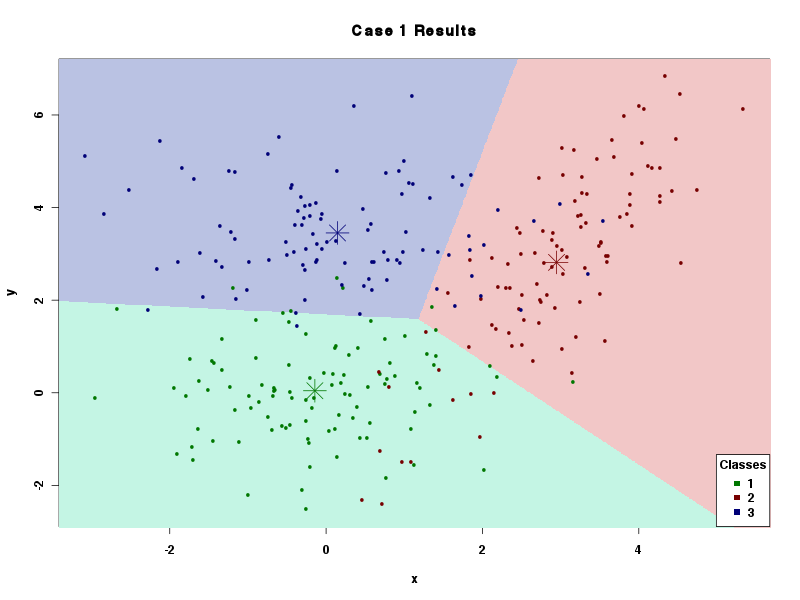
\includegraphics[width=6in]{../plots/case1.eps}
\caption{Results for Case 1: $\mathbf{\Sigma}_i = \sigma^2 \mathbf{I}$}
\end{figure}

\begin{figure}[thb]
\centering
\label{fig:case2-scatter}
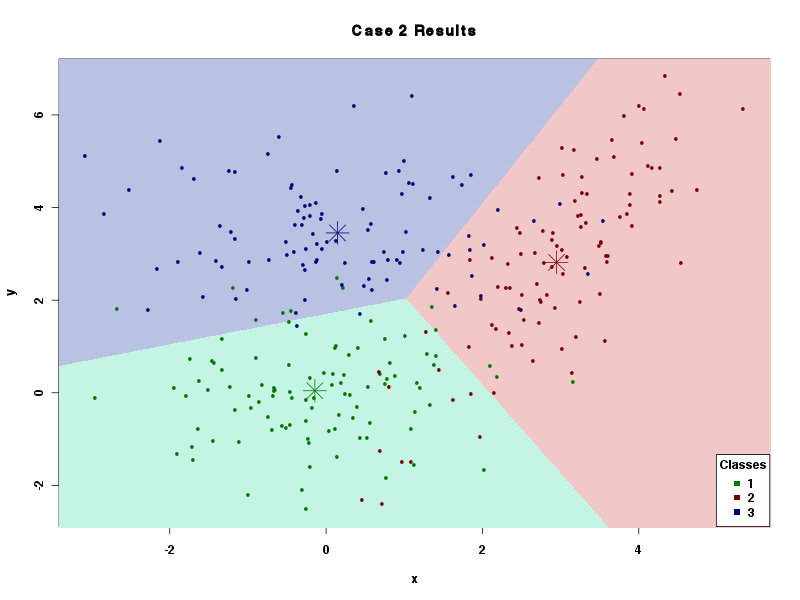
\includegraphics[width=6in]{../plots/case2.eps}
\caption{Results for Case 2: $\mathbf{\Sigma}_i = \mbox{cov}(D)$}
\end{figure}

\begin{figure}[thb]
\centering
\label{fig:case3-scatter}
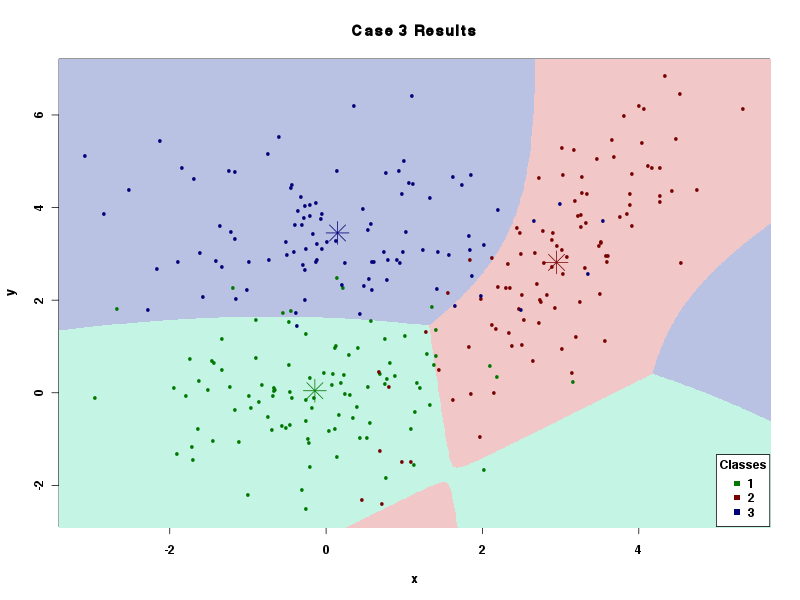
\includegraphics[width=6in]{../plots/case3.eps}
\caption{Results for Case 3: $\mathbf{\Sigma}_i = \mbox{cov}(D_i)$}
\end{figure}

\end{document}
